\documentclass{report}

%%%%%%%%%%%%%%%%%%%%%%%%%%%%%%%%%%%%%%%%%%%%%%%%%%%%%%%%%%%%%%%%%%%%%
%                            Preamble
%%%%%%%%%%%%%%%%%%%%%%%%%%%%%%%%%%%%%%%%%%%%%%%%%%%%%%%%%%%%%%%%%%%%%%
\usepackage[utf8]{inputenc}
\usepackage{textcomp}
% Define page size and margin size
\usepackage{geometry}
\geometry{
    a4paper,
    total={170mm,257mm},
    left=20mm,
    top=20mm,
}
\usepackage{hyperref}
\usepackage{multicol}
\usepackage{wrapfig}
\usepackage[utf8]{inputenc} %to import other docs
\usepackage[DIV=14]{typearea} % to change page size on the fly
\usepackage{pgfgantt} %to insert gantt chart
\usepackage{float} %goddamn figure places
\usepackage{enumitem}
\setlength\parindent{0pt}
% reformat chapter display
\usepackage{titlesec}
\usepackage{listings}
\titleformat{\chapter}{\normalfont\LARGE\bfseries}{\thechapter}{1em}{\LARGE}
\titlespacing*{\chapter}{0pt}{0pt}{10pt}

\counterwithout{figure}{chapter} %global figure counter

\renewcommand{\bibname}{References} % Bibliography? we dont do that here
% Code style
\usepackage{xcolor}
\definecolor{codegreen}{rgb}{0,0.6,0}
\definecolor{codegray}{rgb}{0.5,0.5,0.5}
\definecolor{codepurple}{rgb}{0.58,0,0.82}
\definecolor{backcolour}{rgb}{0.95,0.95,0.92}
\lstdefinestyle{mystyle}{
    backgroundcolor=\color{backcolour},
    commentstyle=\color{codegreen},
    keywordstyle=\color{magenta},
    numberstyle=\tiny\color{codegray},
    stringstyle=\color{codepurple},
    basicstyle=\ttfamily\scriptsize,
    breakatwhitespace=false,
    breaklines=true,
    captionpos=b,
    keepspaces=true,
    numbers=left,
    numbersep=5pt,
    showspaces=false,
    showstringspaces=false,
    showtabs=false,
    tabsize=2
}

\lstset{style=mystyle}
\setlength{\columnsep}{5pt}


\begin{document}
%%%%%%%%%%%%%%%%%%%%%%%%%%%%%%%%%%%%%%%%%%%%%%%%%%%%%%%%%%%%%%%%%%%%%
%TITLE PAGE AND TABLE OF CONTENTS
%%%%%%%%%%%%%%%%%%%%%%%%%%%%%%%%%%%%%%%%%%%%%%%%%%%%%%%%%%%%%%%%%%%%%%
\begin{titlepage}
    \begin{center}
        \vspace*{1cm}

        \vspace{1.5cm}
        \Large
        Department of Electrical Engineering and Computer Science\\
        EECS Senior Design 2021

        \Huge
        \textbf{Modular Garden Monitoring System}

        \vspace{1.5cm}

        \textbf{Team CE12} \\
        {\Large Sadie Gladden, Eric Krenz, Zuguang Liu, Alan Trester}

        \vspace{0.5cm}
        \Large
        April 6, 2021

        \vspace{1.5cm}
        \textbf{Technical Advisor} \\
        {\Large Dr. Zachariah Fuchs}

        \vfill
        %TODO: ADD SIGNATURE SECTION?
        University of Cincinnati\\
        College of Engineering and Applied Science\\
        EECE 5031 CompE Senior Design I - 001

        \vspace{0.8cm}
    \end{center}
\end{titlepage}

%%%%%%%%%%%%%%%%%%%%%%%%%%%%%%%%%%%%%%%%%%%%%%%%%%%%%%%%%%%%%%%%%%%%%%
%DEDICATION??????????
%%%%%%%%%%%%%%%%%%%%%%%%%%%%%%%%%%%%%%%%%%%%%%%%%%%%%%%%%%%%%%%%%%%%%%
% We dedicate this report to ourselves for surviving zoom senior design class with Purdy. Big shout-out to her cat(SABRIIIIIIIIIIIIIINNNNNNNNNNAAAAAA), the old rotary phone that would always ring during class, and her mac from 2003.
\newpage
\section*{Acknowledgements}
We would like to sincerely thank the following individuals:
\begin{itemize}
    \item
          \textbf{Dr. Carla Purdy} for your continued guidance and wisdom throughout the Senior Design process.
    \item
          \textbf{Dr. Zach Fuchs} for supporting, advising, teaching, and dealing with us throughout the creation and development of this project.
    \item
          \textbf{Hive 13 Makerspace} for providing work space and equipment that was vital to the development of our prototype.
\end{itemize}

%%%%%%%%%%%%%%%%%%%%%%%%%%%%%%%%%%%%%%%%%%%%%%%%%%%%%%%%%%
%TOC
%%%%%%%%%%%%%%%%%%%%%%%%%%%%%%%%%%%%%%%%%%%%%%%%%%%%%%%%%%%
\tableofcontents
%TODO : ADD FIGURE LIST?
%TODO : ADD FIGURES W/ DESCRIPTIONS IN BODY/APPENDIX

%%%%%%%%%%%%%%%%%%%%%%%%%%%%%%%%%%%%%%%%%%%%%%%%%%%%%%%%%%%%%%%%%%%%%%
%ABSTRACT
%%%%%%%%%%%%%%%%%%%%%%%%%%%%%%%%%%%%%%%%%%%%%%%%%%%%%%%%%%%%%%%%%%%%%%
\newpage
\section*{Abstract}
The MGMS is an IoT solution to help homeowners, garden enthusiasts, and farmers care for their lawns and gardens in a more informed and effective way while also reducing wasteful water usage. This proof-of-concept system designed over the 2020/2021 fall and spring semesters utilizes an AVR microcontroller and IEEE 802.15.4 wireless communication to provide real-time and historical information about outdoor or indoor environmental conditions while providing customized recommendations for optimal plant care.


%%%%%%%%%%%%%%%%%%%%%%%%%%%%%%%%%%%%%%%%%%%%%%%%%%%%%%%%%%%%%%%%%%%%%%
%PROBLEM STATEMENT
%%%%%%%%%%%%%%%%%%%%%%%%%%%%%%%%%%%%%%%%%%%%%%%%%%%%%%%%%%%%%%%%%%%%%%
\chapter{Introduction}
The purpose of this report is to divulge in its entirety, the process followed to fulfill all requirements of EECE5031/5032–Senior Design, at the University of Cincinnati’s College of Engineering and Applied Science. The culminating project is a proof-of-concept modular garden monitoring system.

\section{Problem/Need}

Lawns and gardens are one of most essential elements for the typical American home. A survey conducted by National Association of Landscape Professionals in 2019 shows that 79 percent of American families value lawns when renting or buying a home, and about one in three Americans garden in their yards multiple times a week\cite{noauthor_new_2019}. \\

Consequently, there is a constantly high demand of water for use in lawns and gardens. Per the United States Environmental Protection Agency, about 48 gallons of water is devoted for this use per family per day. Across America, nearly 1/3 of all residential water is used for landscaping irrigation totaling an estimated 9 billion gallons per day\cite{epa_outdoor_nodate}. In a world undergoing climate change with consistent annual water shortages and wildfires in many parts of the world, wasteful water usage is simply irresponsible and unacceptable. \\

The issue of wasteful irrigation is not being addressed as actively as it deserves to be. Although  younger  generations  of  Americans  tend  to  value  lawns  and  gardens  even  more than older generations, more than half of young people failed quizzes on proper landscape care and nearly 7 out of 10 young people wish to see further improvement in their lawns\cite{epa_drought_nodate}.Uninformed (and in turn, irresponsible) lawn care may significantly contribute to the amount of wasteful water usage happening every day.

A 21st-century solution is needed to help new homeowners care for their lawns and gardens in a more informed and effective way while reducing the amount of wasteful water usage that is accounted for by residential lawn care and irrigation. \\

\section{Solution}

Originated from the Internet of Things (IoT) concept, the Modular Garden Monitoring System (MGMS) is a proposed solution that will be able to provide real-time and historical information about environmental conditions. Simply having detailed information on-hand will allow homeowners to make more informed decisions on the types of plants to keep in their gardens as well as when and how much to water them. Internet connectivity can take decision making to the next level by being able to crowd-source gardening recommendations and consider local weather predictions for watering. Further system expansions can introduce features such as automatic watering to take work from homeowner's shoulders while reducing human error in the garden care process. Finally, a smart design will allow the system to be flexible and applicable in a variety of scenarios varying with garden size and irrigation needs and even between residential and industrial settings. This senior design project will focus on creating a proof-of-concept baseline system to report and access environmental data. The user interface will be built in such a way that will enable smooth addition of the smart features discussed above.

\newpage
\section{Credibility}

\textbf{Alan Trester} is an Electrical Engineering student with co-op experience in software, hardware, and manufacturing engineering roles through GE Aviation Systems. He has a strong passion for technology, design, and "making". After graduating he will begin full-time work as an Electrical Engineer with Raytheon Missile \& Defense in Tucson, Arizona.\\

\textbf{Eric Krenz} is a Computer Engineering student whose past co-op experience was in hardware, software development, and cybersecurity. He has a passion for engineering, technology, and making the world a better place. Post graduation he will begin his career at Epic Systems in Madison, Wisconsin. \\

\textbf{Sadie Gladden } is a Computer Engineering student with co-op experience in software developement, user interface creation, game engine developement, computer graphics, and cloud solutions through Siemens PLM and Siemens Healthcare GmbH. She enjoys exploring the relationship between hardware and software and exploring the connection and overlap of technology and medicine.\\

\textbf{Zuguang Liu} is an Electrical Engineering student who has past Co-op experience in industrial system design, embedded system hardware design, and simple machine learning implementation. After finishing a Bachelor's Degree with an Embedded Systems minor, he will continue to pursue a Master's Degree in Electrical Engineering.\\

Team member responsibilities often overlapped during the development of the MGMS. Overall however, task assignments were chosen based on each members personal engineering strengths and abilities. Figure \ref{fig:TeamChart} illustrates each team member's experience and project focus for the development of the MGMS. This image was originally presented during the design planning phase of the project.\\

\begin{figure}[H] %H means keep figure here
    \centering
    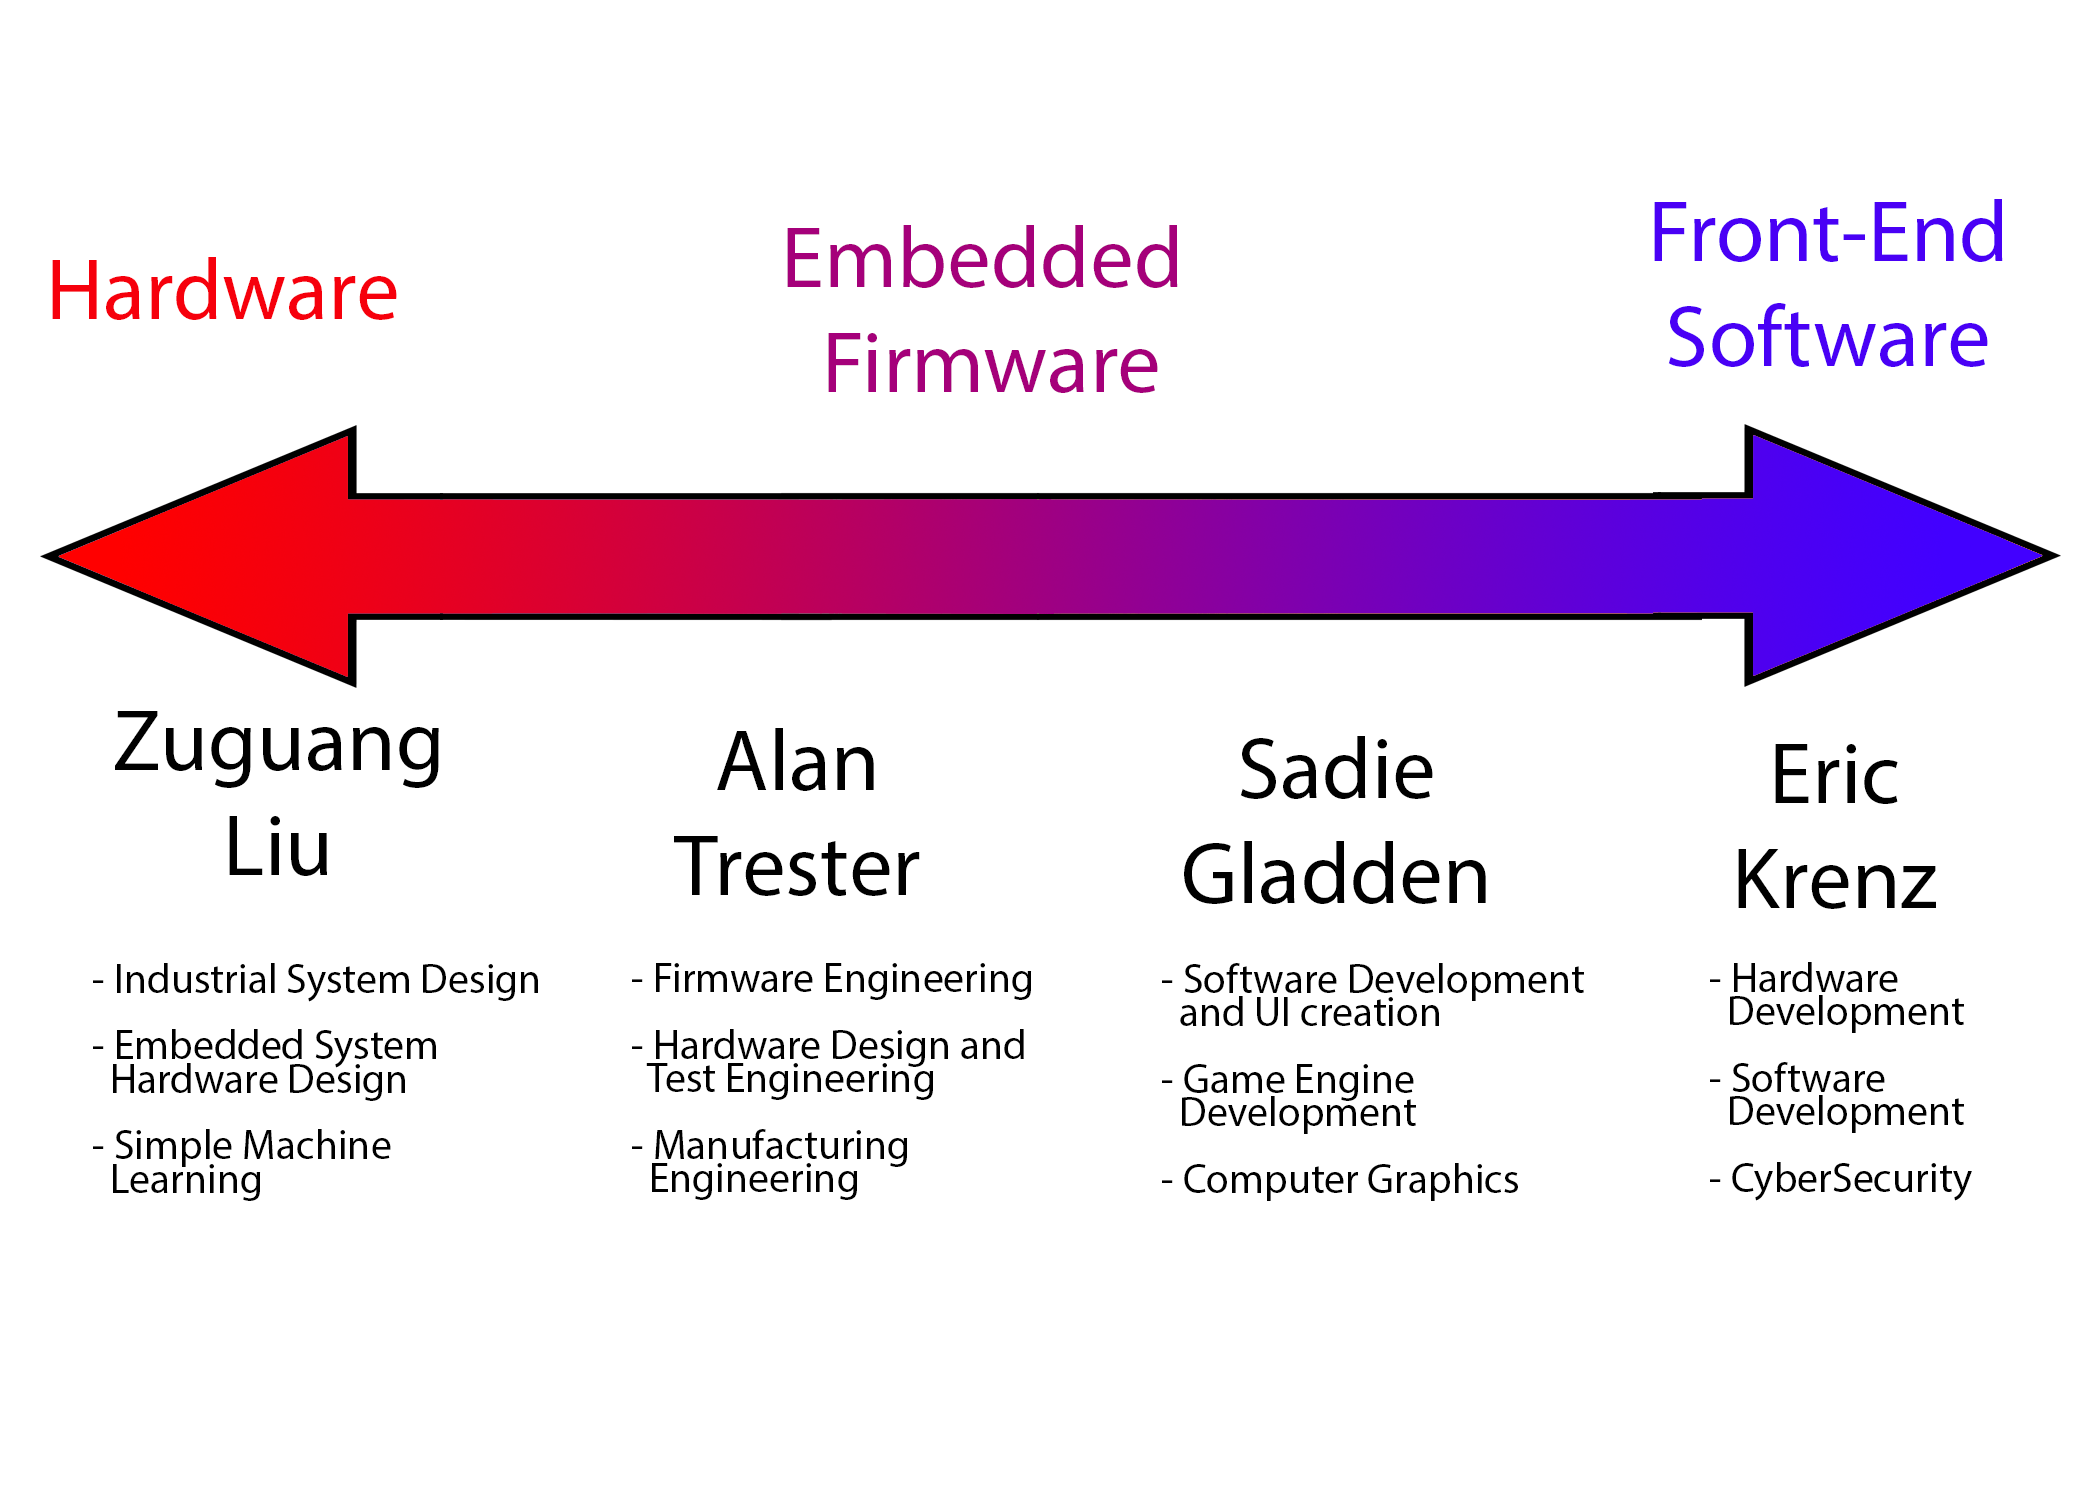
\includegraphics[height=3.5in]{PNGs/Arrow.png}
    \caption{Team members past experience, specializations, and credibility for this project.}
    \label{fig:TeamChart}
\end{figure}

\textbf{Dr. Zachariah Fuchs} (\href{fuchsze@ucmail.uc.edu}{fuchsze@ucmail.uc.edu}) is the professor for Introduction to Mechatronics. He has extensive knowledge on embedded system design, sensor fusion, robotics and control systems. His areas of expertise make him a good source of advice on anything from the top-level architecture of the system to individual component choices and design\\

\section{Project Goals and Brief Methodology}
Our proposed solution is a modular garden monitoring system that will be able to provide real-time and historical information about environmental conditions such as soil moisture, temperature, sunlight, humidity, and so on. This is a depth of information that is not necessarily available on existing products; Simply having this detailed information on-hand will allow homeowners to make more informed decisions on the types of plants to keep in their gardens as well as when and how much to water them. This removes the need for a strong knowledge in horticulture for effective results as well as taking water conservation up a notch. The intended proof-of-concept system will be able to report on and present real-time and historical data on environmental conditions. Project work will focus on the system's wireless communications capabilities, sensor interface, and user interface platform.\\

The desired characteristics of the MGMS were defined in an attribute table and identified as objectives, constraints, functions, or means. This is presented in Figure \ref{fig:Attribute}. These identified attributes are referenced throughout the design planning and testing process.
\begin{figure}[H] %H means keep figure here
    \centering
    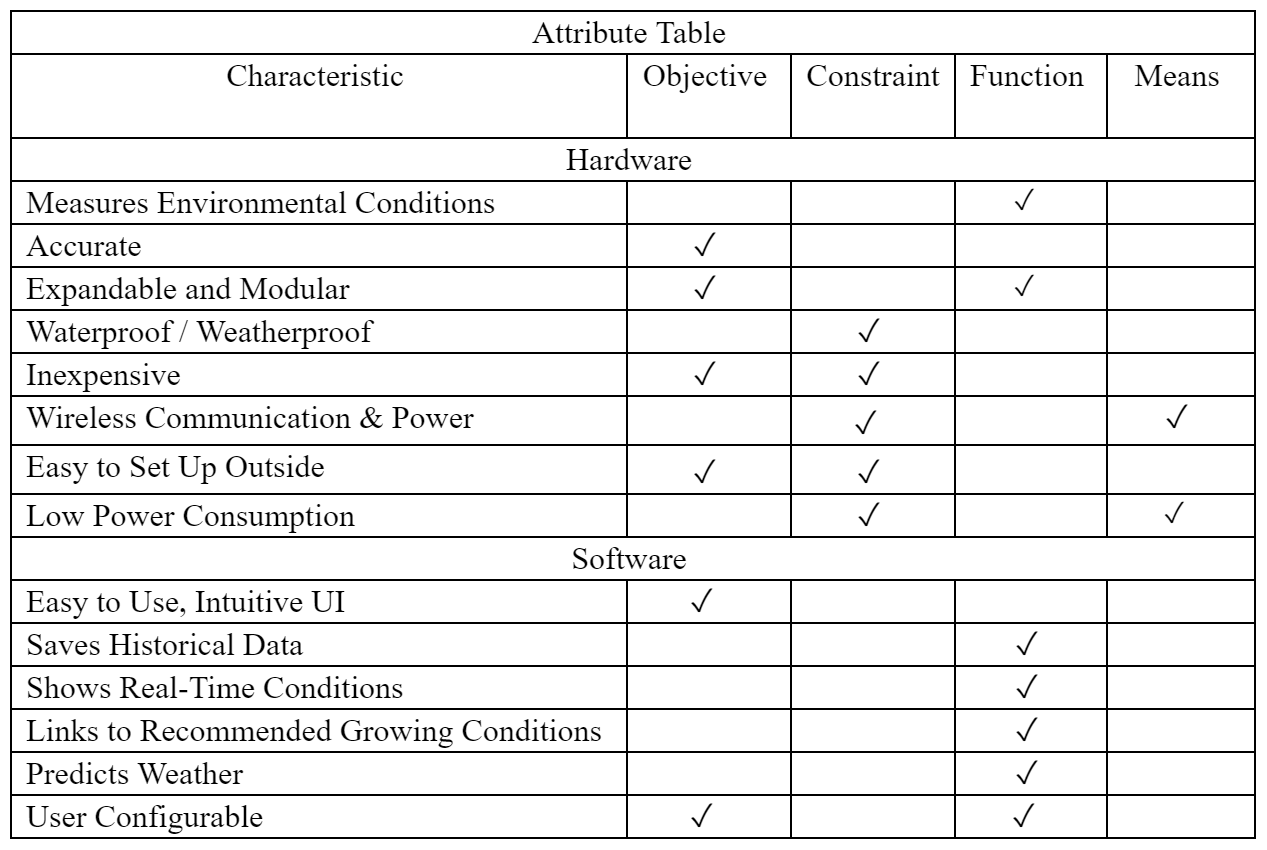
\includegraphics{PNGs/AttributeTable.PNG}
    \caption{Attribute Table used during the design decision making process.}
    \label{fig:Attribute}
\end{figure}
This kind of system can be made using a simple embedded system architecture. A basic microcontroller (or family of controllers), which can be chosen to be used throughout the system modules, will be capable of any combination of reading inputs from sensors, sending information, receiving information, and interacting with actuators such as solenoid valves to control water flow. The heart of the system lies in the radio modules, such as Zigbee radios, which allow for full modularity and good wireless range. Finally, the forward-facing system UI can be hosted on a tiny computer such as a Raspberry Pi.\\

%%%%%%%%%%%%%%%%%%%%%%%%%%%%%%%%%%%%%%%%%%%%%%%%%%%%%%%%%%%%%%%%%%%%%%
%DISCUSSION
%%%%%%%%%%%%%%%%%%%%%%%%%%%%%%%%%%%%%%%%%%%%%%%%%%%%%%%%%%%%%%%%%%%%%%
\chapter{Discussion}

\section{Project Concept}
A garden monitoring system such as the one we are proposing is not a novel idea: several products already exist within the consumer and industrial farming markets with similar approaches towards data collection. The Onset HOBOnet system is a web-enabled data-collection solution for industrial farmers. While these systems are very popular and provide good results, with accessible user interfaces and informative data visualization, they are too expensive for consideration by homeowners and don’t have the necessary features such as garden suggestions to be applicable in that market \cite{onsethobo}. The Edyn Garden Sensor was a consumer-targeted system that aimed to tackle the same problems as the MGMS, unfortunately the product was burdened with limited modularity and expandability as well as a poorly designed app interface \cite{edyn}. Characteristics of both products are analyzed and, along with interviews and the team’s own expectations, are used to set a reasonable objectives baseline for the new system.\\

A pairwise comparison chart is used to identify priorities among certain attributes that are identified in Figure \ref{fig:Attribute} above. Again, these attributes are considered throughout the design process and are presented in Figure \ref{fig:Pairwise}.\\

\begin{figure}[H] %H means keep figure here
    \centering
    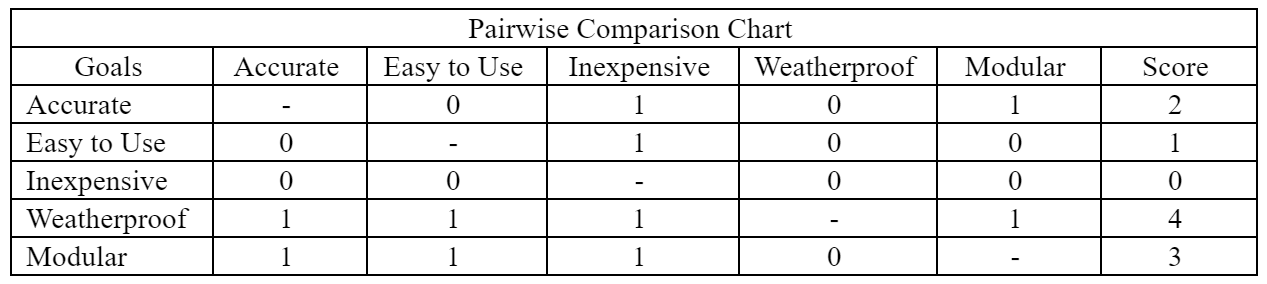
\includegraphics{PNGs/PairwiseComparison.PNG}
    \caption{Pairwise Comparison Chart for the design process of our prototype.}
    \label{fig:Pairwise}
\end{figure}

\newpage
\section{Design Objectives}
The end-goal of this project is to develop a proof-of-concept marketable product to functionally address the issues previously discussed in the problem statement: Poor gardening practices and Water conservation. To aid the project development structure, two objective trees are created, referencing identified attributes and priorities from before, for the hardware and software components of the system seperately. These charts are presented in Figures \ref{fig:SWTree} and \ref{fig:HWTree} respectively.
\begin{figure}[H] %H means keep figure here
    \centering
    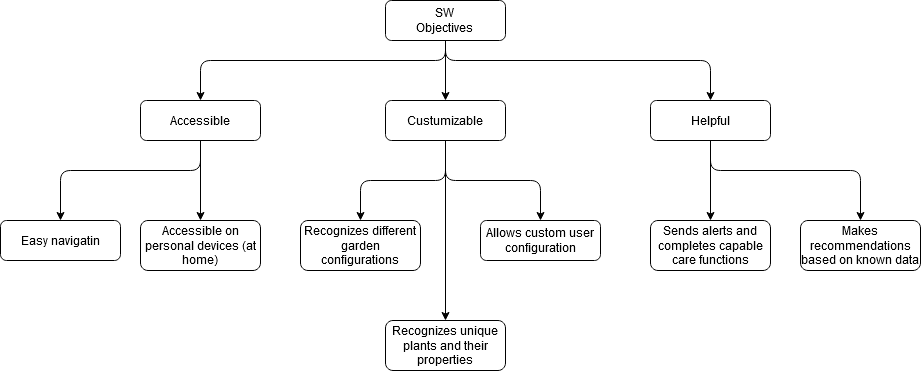
\includegraphics[height=2.75in]{PNGs/SW_Objective_Tree.png}
    \caption{Software Design and Implementation Objective Tree for the design priorities of creating a product that is Accessible, Customizable, and Helpful for the consumer.}
    \label{fig:SWTree}
\end{figure}
\begin{figure}[H] %H means keep figure here
    \centering
    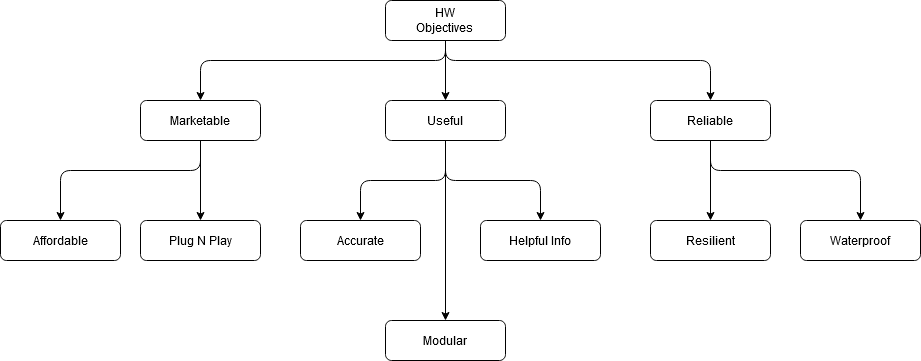
\includegraphics[height=2.75in]{PNGs/HW_Objective_Tree.png}
    \caption{Hardware Design and Implementation Objective Tree for the design properties of being Marketable, Useful, and Reliable for the consumer.}
    \label{fig:HWTree}
\end{figure}
\newpage
As a consumer-based product, we define a qualitative functionality as the end goal: supporting users to care for their gardens and reasonably complete automated garden care when enabled. Aside from hardware sensor specifications, quantitative requirements are not realistic for this project, especially considering the time and resource limitations associated with the 2021 senior capstone framework. For example, assessing the effectiveness of the MGMS in improving garden yield would require long-term testing in a dedicated space, which would not be possible to complete following a semester timeline and difficult in a virtual collaborative environment.\\

Initial project requirements will be wholly qualitative outside of hardware requirements and will follow previously identified objectives. For the intended system demonstration in April 2020, system effectiveness will not be tested in lieu of testing for intended system functionality and correct hardware performance. With correct hardware performance, system functionality can be more easily tweaked in software to improve overall system performance once that testing occurs. Because of this, the described level of testing is acceptable for a simple demonstration in April.\\

Qualitative system attributes such as ''ease of use'' will be assessed separately during testing in a variety of ways. Timeline and resource permitting, surveys and qualitative analysis can be conducted . This testing will later be defined during the development process.\\

The intended system functionality is as follows:

\begin{enumerate}[label=\alph*.]
    \item
          Promotes green spaces by lowering the learning curve of home lawn or garden care.
          \begin{itemize}
              \item
                    Real-time vital statistics
              \item
                    User configurable setup
              \item
                    Modular to mold to a variety of use-cases
          \end{itemize}
    \item
          Solves the common problem of garden over-watering to conserves water
          \begin{itemize}
              \item
                    Control system to keep garden soil moisture at healthy levels
              \item
                    Predicts weather patterns and only automatically waters when needed
          \end{itemize}
\end{enumerate}
\newpage
\section{Methodology/Technical Approach}
The definition of the product inherently makes the design an embedded system that requires multi-disciplinary knowledge and skills. Thus, we use the \textbf{strategy of design decomposition} to reduce the complexity of the problem to match each team member's expertise. Each hardware device (including sensors, controllers and actuators) will be set-up and tested individually during design prototyping, then combined into a complete system and tested afterwards. The UI software does not depend on hardware as much, so the front-end development is performed separately, while having tasks and deadlines in the same pace as the hardware development, such that the whole system can be defined and prototyped synchronously. \\

Using a strategy of design decomposition provides several benefits to the project development efforts, the biggest of which is acting as a ``cushion'' for possible issues that may arise during development and prototyping. Design decomposition means that each system component is evaluated separately, removing dependency on any one component for the final system function. This way, if an issue arises during development, a component or design can be adjusted without affecting the major development of the project as a whole. This is especially important because of the many different sensors and communication technologies being considered for the project. It is likely that sensor accuracy or communication performance may arise as an issue for individual components. Thanks to a design decomposition strategy, these issues will be able to be solved without much consequence.\\

A baseline system design is created to satisfy the desired project functionality and attributes. This design is shown in Figure \ref{fig:SystemDiagram} as a broken down view showing the three system components that were planned to be developed during the timeline of this project. Figure \ref{fig:NetworkDiagram} shows a network topology view of the developed system.\\

\begin{figure}[H] %H means keep figure here
    \centering
    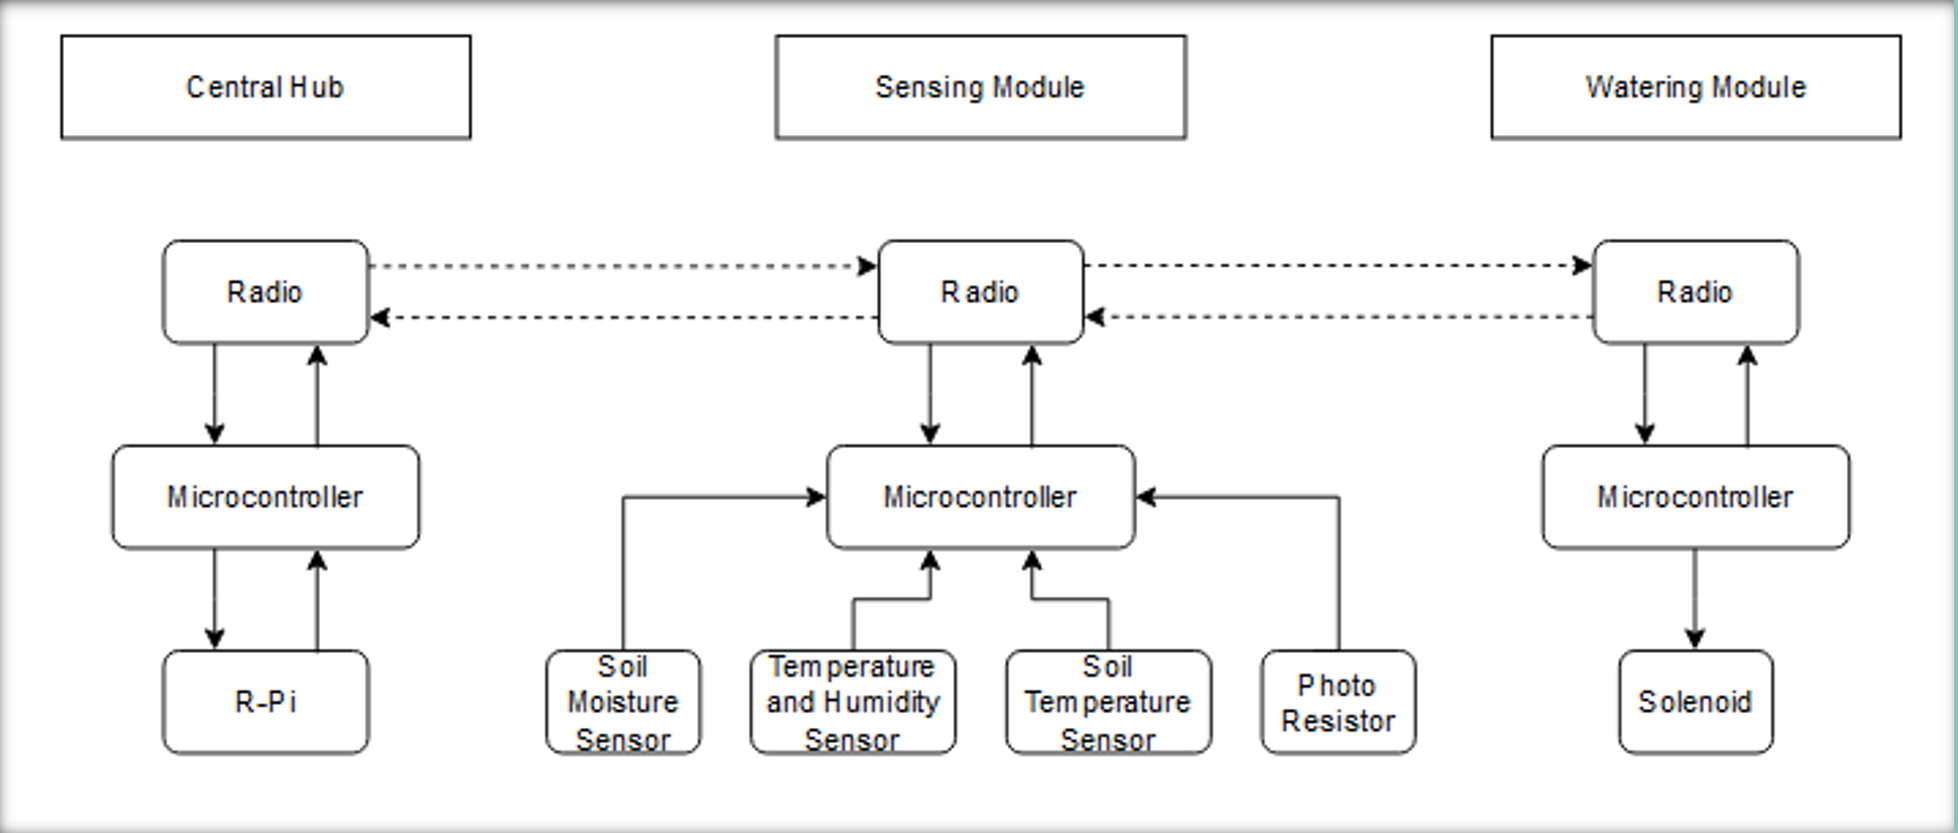
\includegraphics[height=2.75in]{PNGs/SystemDesign.PNG}
    \caption{Overall System Design Overview of the prototype.}
    \label{fig:SystemDiagram}
\end{figure}

\begin{figure}[H] %H means keep figure here
    \centering
    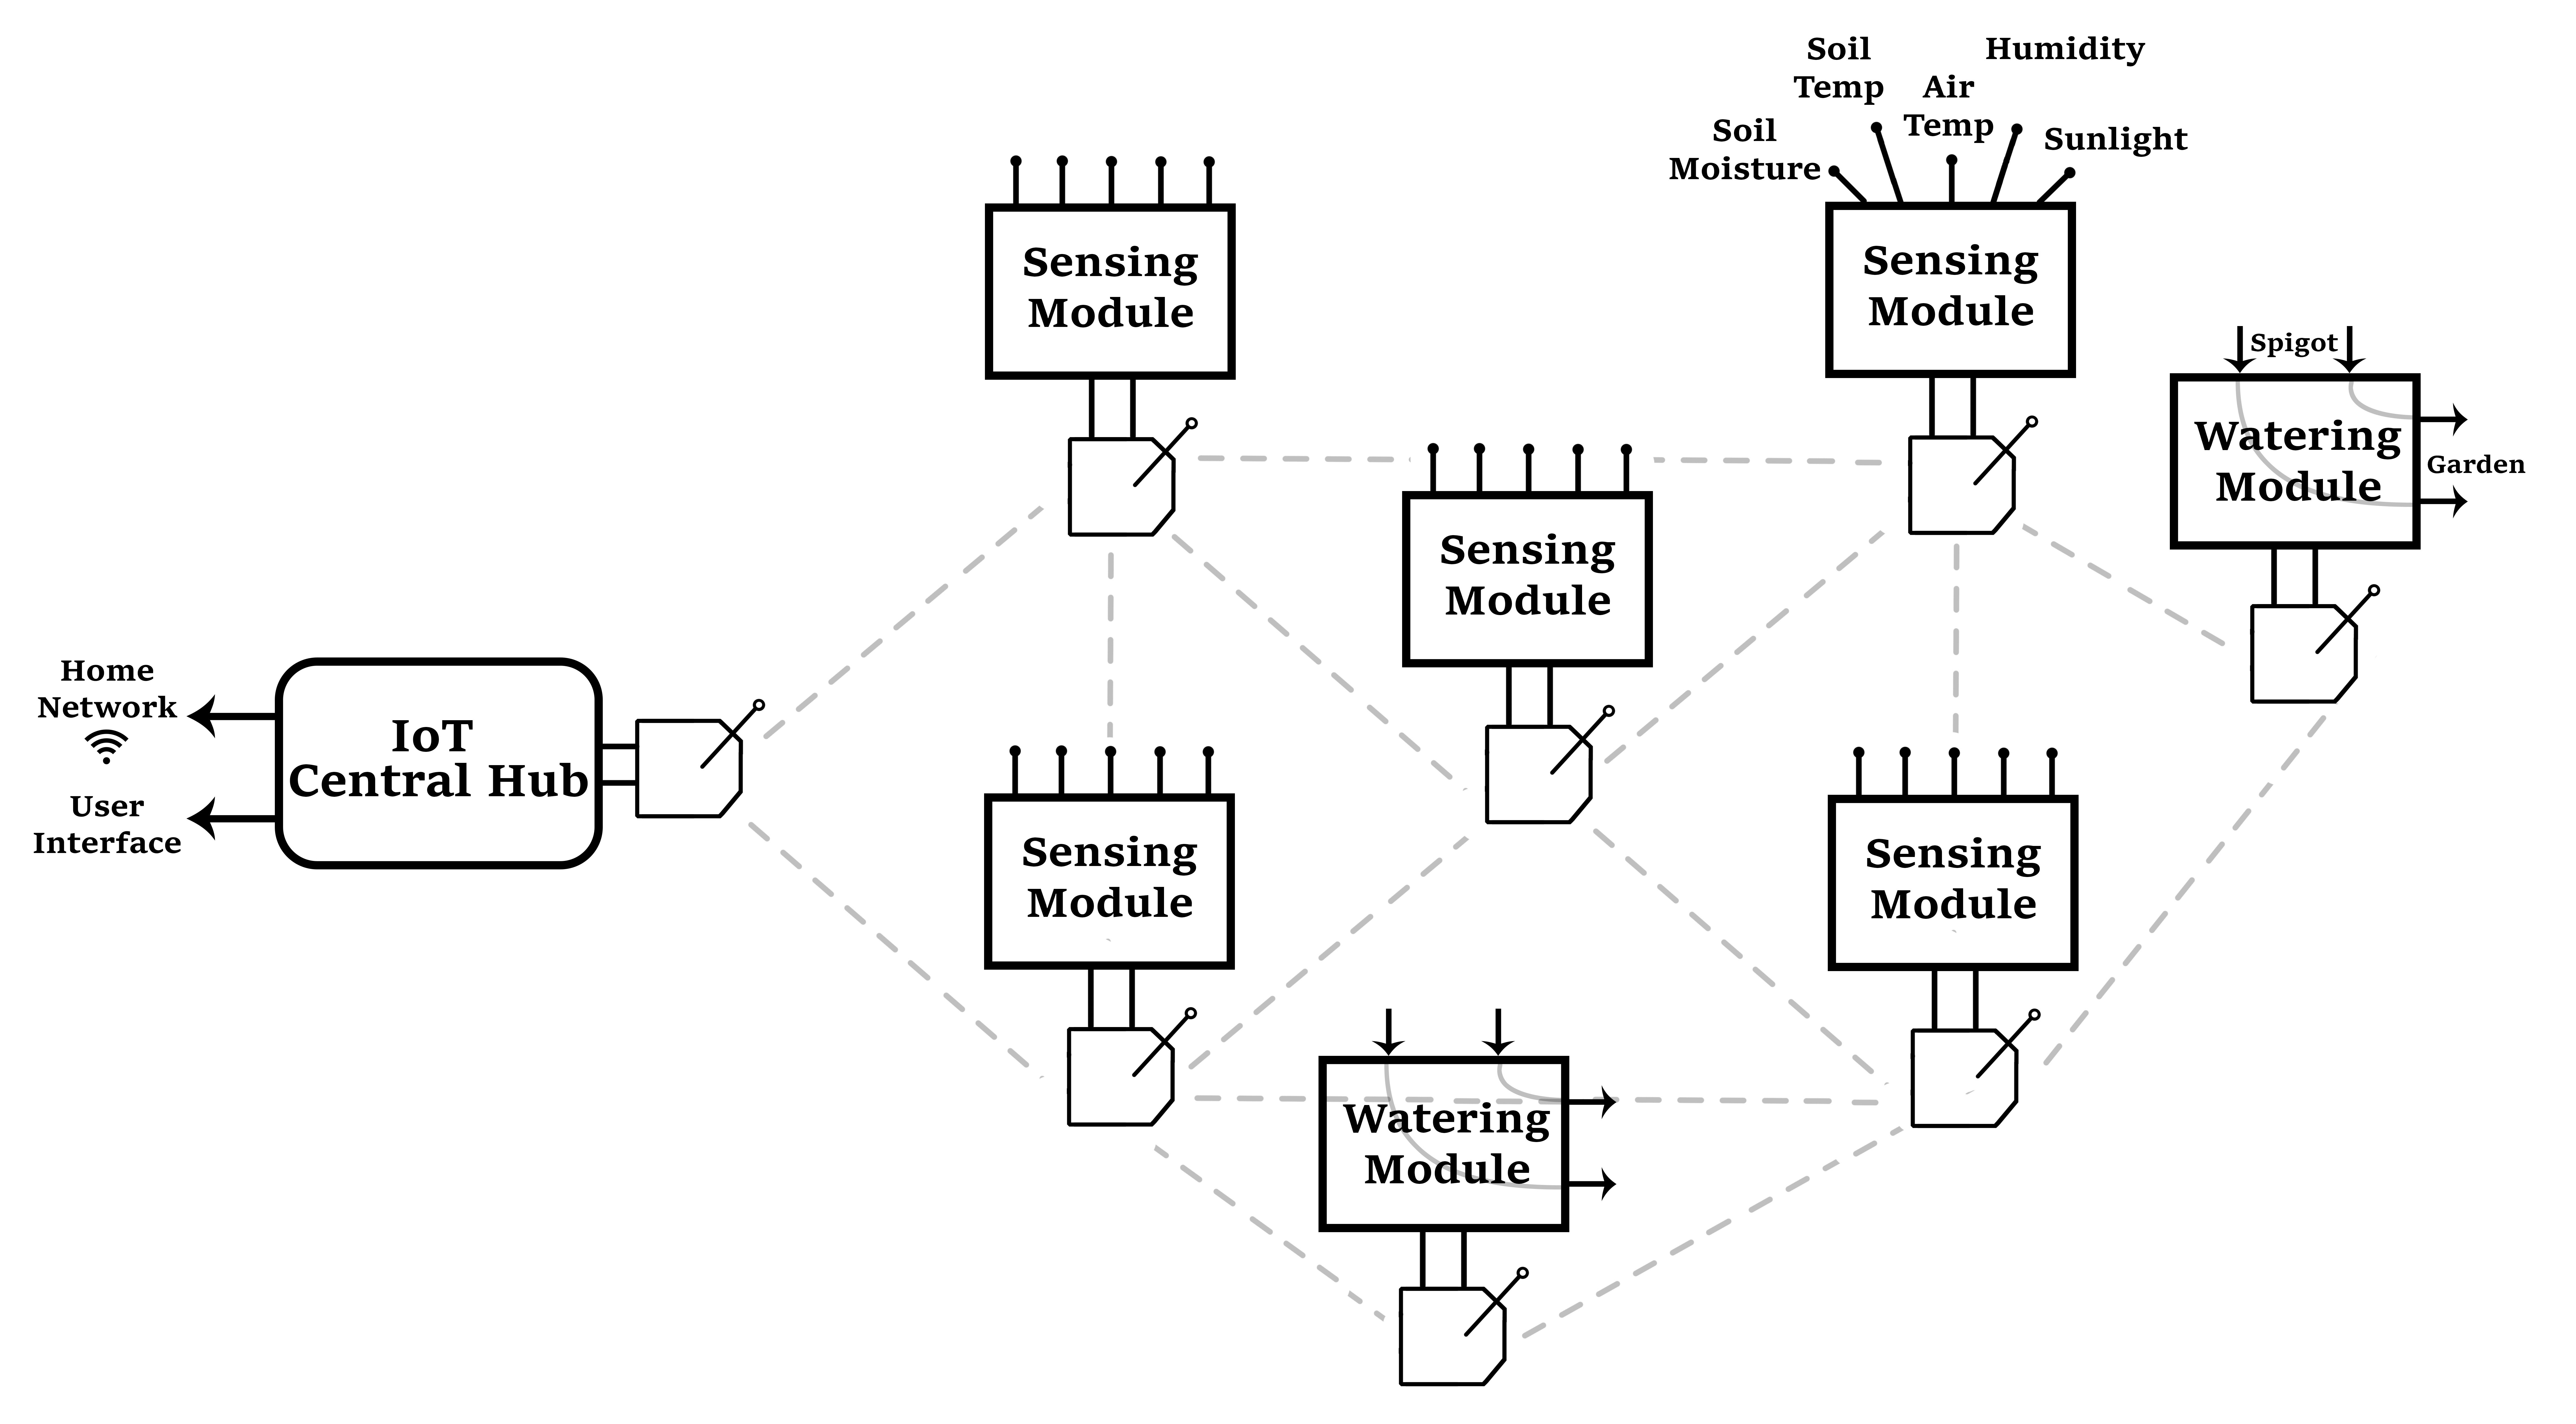
\includegraphics[height=3.5in]{PNGs/System Diagram.jpg}
    \caption{Network Topology view of the Completed System.}
    \label{fig:NetworkDiagram}
\end{figure}

The MGMS system utilizes a modular design consisting of a central hub which will wirelessly connect to multiple sensing and watering modules that can be placed around a garden or house. The hub will host the central user interface and allow for customizing different garden setups. The hub software will make decisions based on the user configuration to control connected field modules in order to continuously monitor and water the garden. The user interface will be able to alert the user to garden events and make suggestions based on information available on the internet. The most important feature of the system should be modularity in freedom to interface a variety of system components in many different configurations.\\

To create a system following the presented design, tools such as a pairwise comparison chart, morphological chart, and decision tables were used to make design decisions in the definition and development phases of this project. The morphological chart, which was used to identify system components for prototyping and production is shown in Figure \ref{fig:Morph} below.
\begin{figure}[H] %H means keep figure here
    \centering
    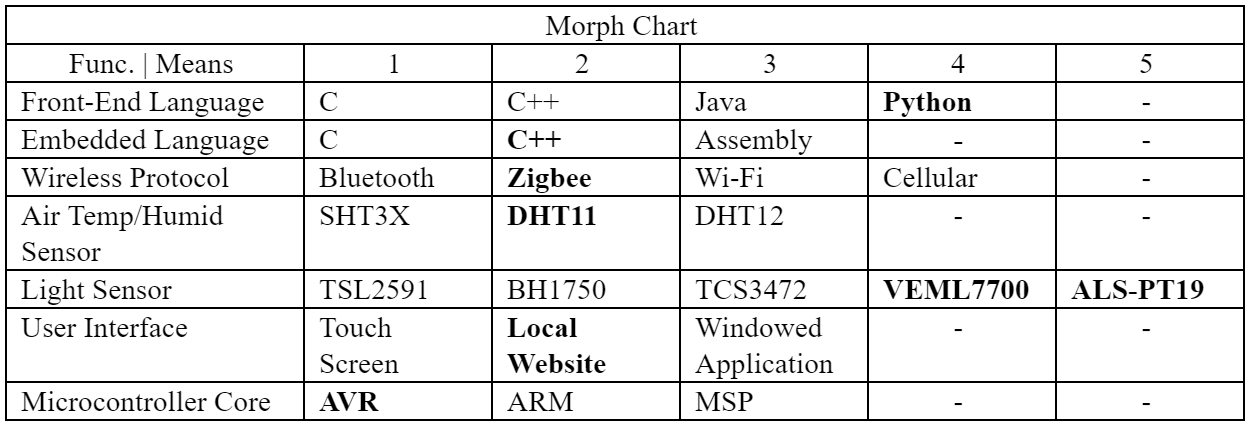
\includegraphics{PNGs/MorphChart.PNG}
    \caption{Morph Chart that shows various design decisions that were made throughout the creation of the MGMS prototype.}
    \label{fig:Morph}
\end{figure}

\section{Standards}
The development of the project conforms to various kinds of professional standards in the embedded system and IoT industry for the sake of security, readability and compatibility. \\

The product uses I2C bus and protocol for intra-board communication between devices, and uses Zigbee as inter-module wireless protocol. I2C (Inter-Integrated Circuit) is a synchronous serial communication bus invented by Philips Semiconductor (now NXP Semiconductors) \cite{noauthor_um10204_2014} and widely used by current IC's in the market. Zigbee is a protocol developed by Zigbee Alliance based on IEEE-802.15.4 standard. IEEE-802.15.4 defines a two-layer architecture for low-data-rate wireless personal area networks (WPAN) \cite{noauthor_ieee_2016}, while Zigbee enhances it with two software layers \cite{zigbee_alliance_zigbee_nodate}. Together they form a mature model to implement IoT concepts. \\

Additionally, electrical diagrams such as circuit schematic and PCB (printed circuit board) layout will be documented digitally in CAD (computer-aided design) software with standard rules and symbols built in. Common circuit diagram and PCB standards are specified in \cite{noauthor_ieee_1993} and \cite{noauthor_ieee_2020}. \\

Finally, standards used in the software development, such as syntax and architecture, are based on specific dependencies, and they must be obeyed in order for the source code to successfully build or run. These standards are flexible in the development phase and will are chosen by the team members during project development.

\newpage
\section{Final System Design}
Through the development process, a final system prototype and production design were created. The physical prototype created covered the following system components.
\begin{itemize}
    \item
          \textbf{Central Hub}
          \begin{itemize}
              \item
                    Wireless-to-Direct Serial Interface
              \item
                    Raspberry Pi Platform
          \end{itemize}
    \item
          \textbf{Sensor Hardware Module}
          \begin{itemize}
              \item
                    Direct-Wireless Serial Interface
              \item
                    Arduino Platform (ATMega328p)
              \item
                    Hardware Sensor Interface
              \item
                    Embedded C Software Enabling Full Module Functionality
          \end{itemize}
    \item
          \textbf{Wireless Communication Framework}
          \begin{itemize}
              \item
                    Serial Communication Datastream Standards
              \item
                    802.15.4 Firmware and Standard Configuration
          \end{itemize}
    \item
          \textbf{User Interface}
          \begin{itemize}
              \item
                    Python-Programmed Serial Interface for Raspberry Pi Connections
              \item
                    Python-Programmed Graphical User Interface
              \item
                    Data Visualizaion
          \end{itemize}
\end{itemize}

Figure \ref{fig:Prototype} shows a photograph of the completed sensor hardware module prototype. In the photograph, it is easy to identify the XBee wireless radio interface, soil sensor interface, and power system.\\

\begin{figure}[H] %H means keep figure here
    \centering
    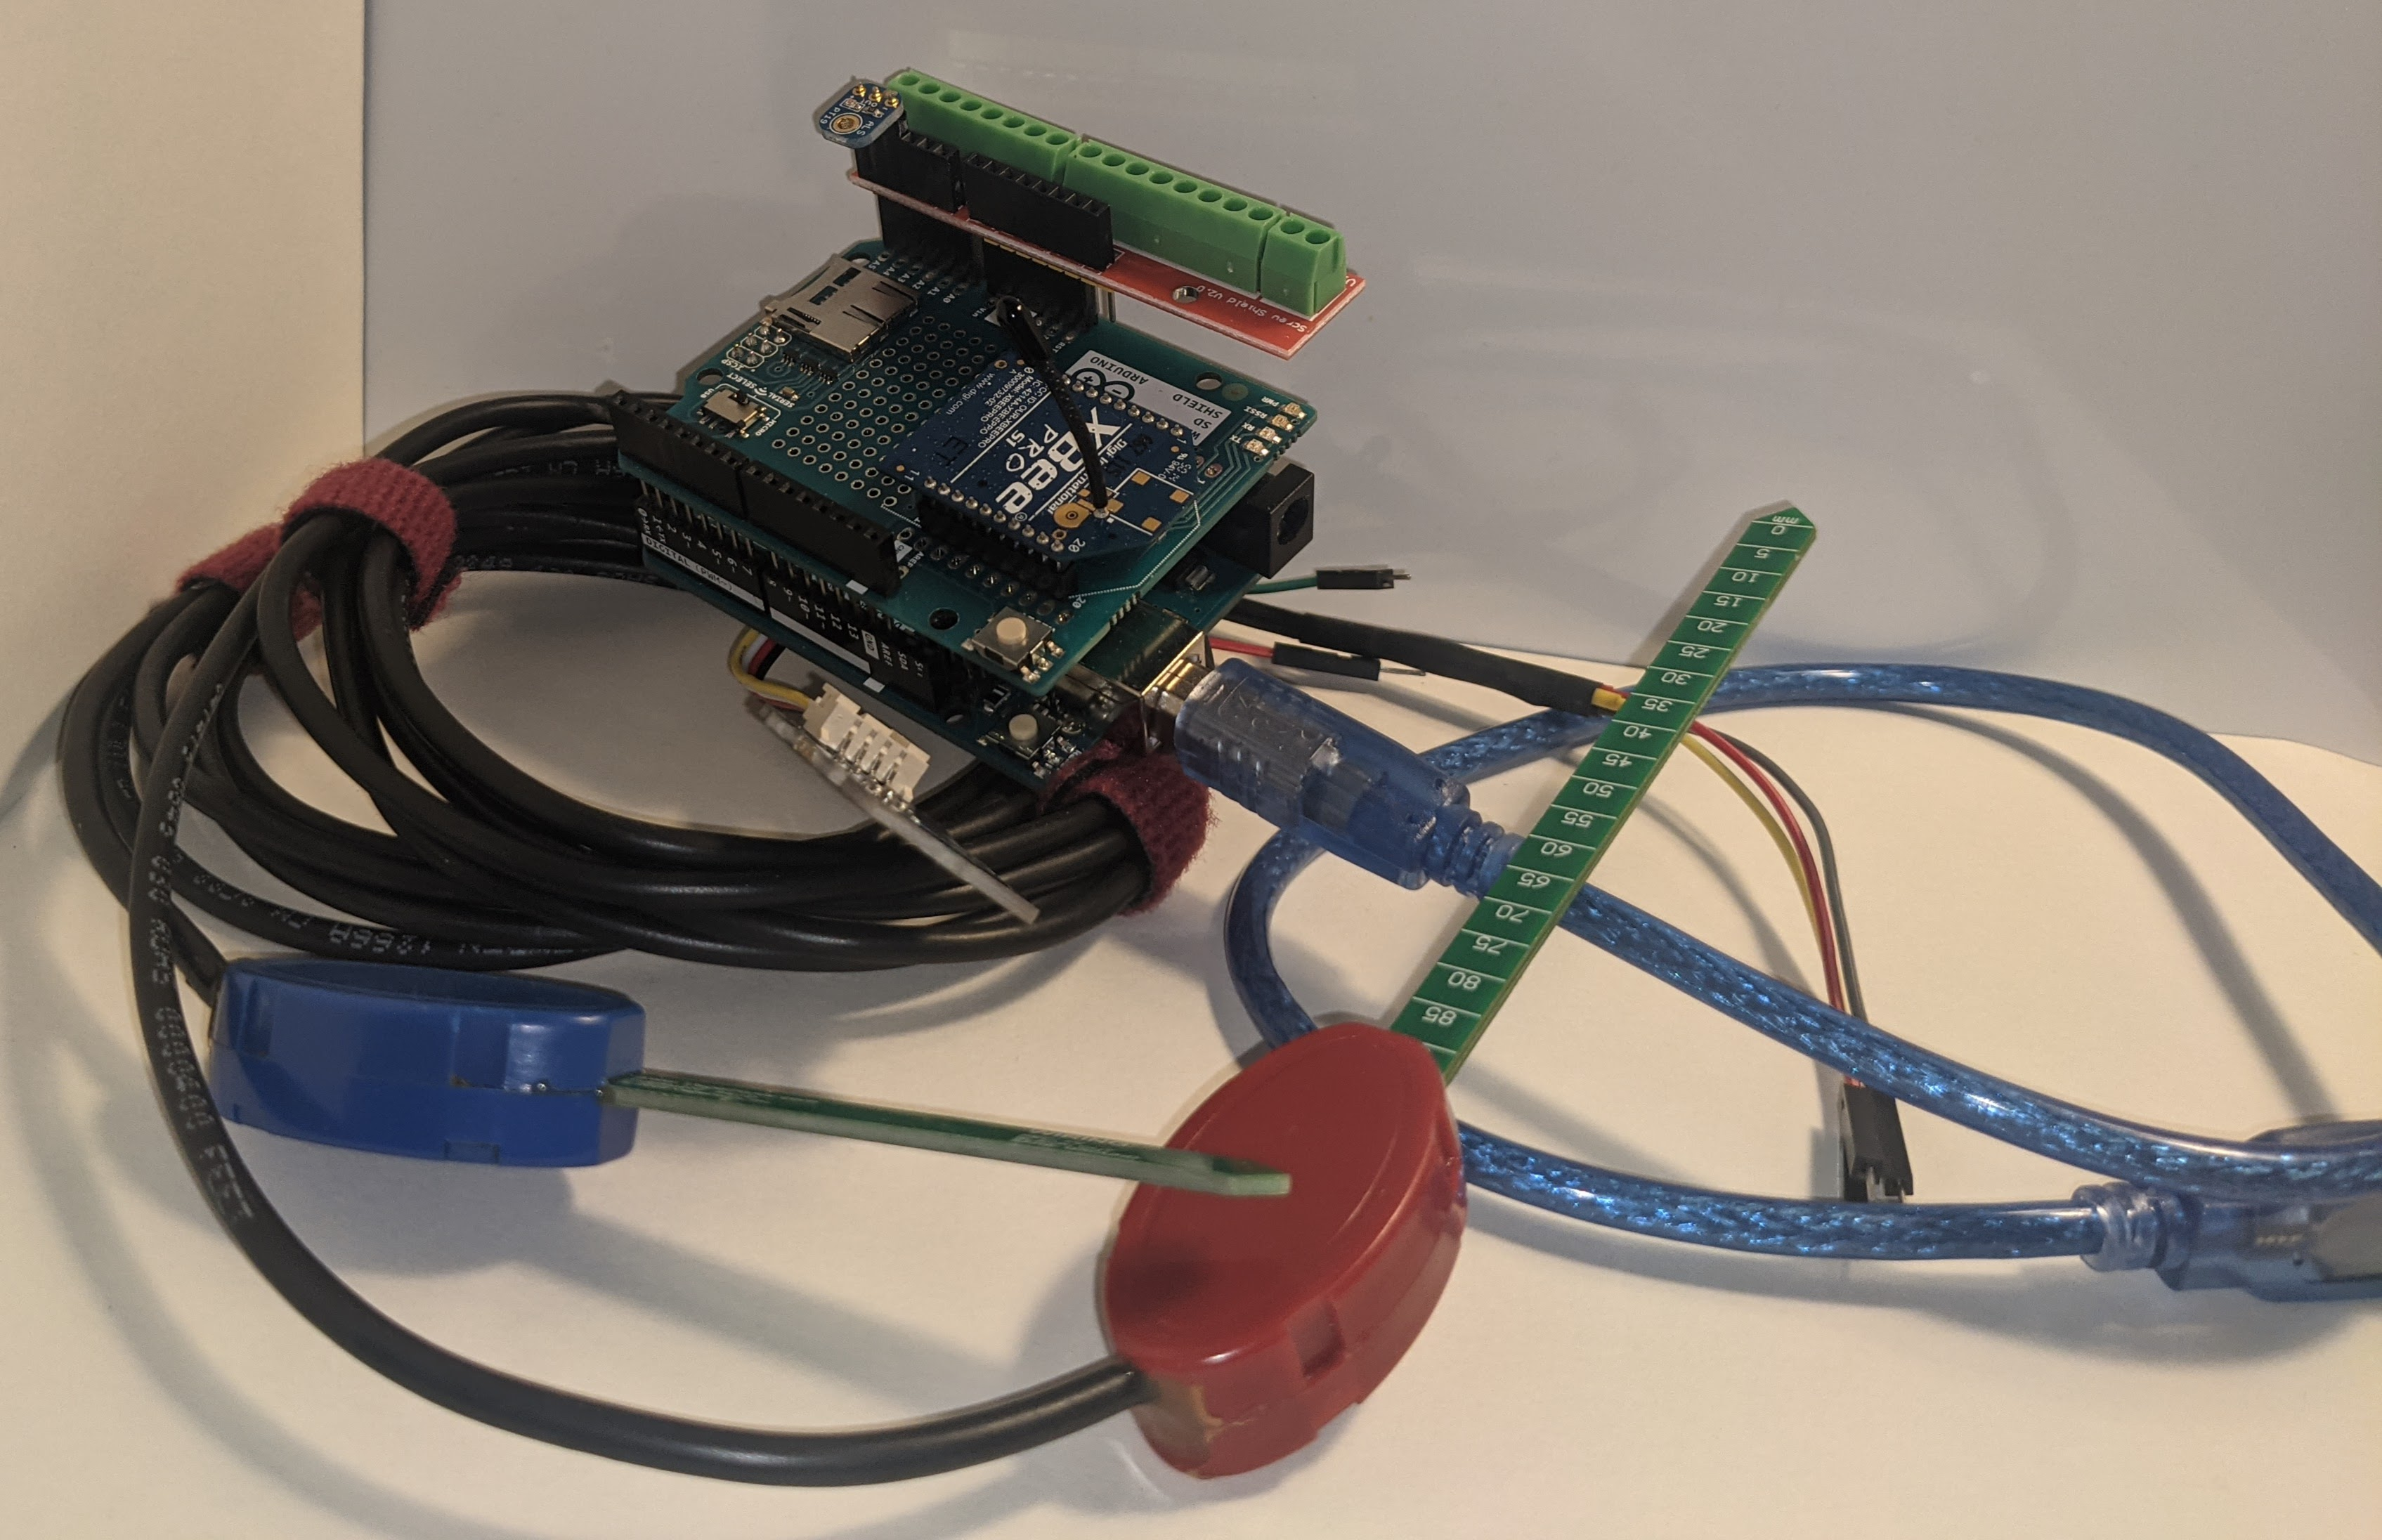
\includegraphics[height=4in]{PNGs/Prototype.jpg}
    \caption{Fully Completed Prototype of the MGMS Hardware Sensor Module.}
    \label{fig:Prototype}
\end{figure}

Complimenting the central hub hardware, a graphical user interface and historical data visualization system were developed. This system allows for user interaction with components interfaced within the wireless network and was partially used for hardware testing during performance evaluation. Figures \ref{fig:GUI} and \ref{fig:Graph} show the main UI menu and sample data chart respectively.\\

\begin{figure}[H] %H means keep figure here
    \centering
    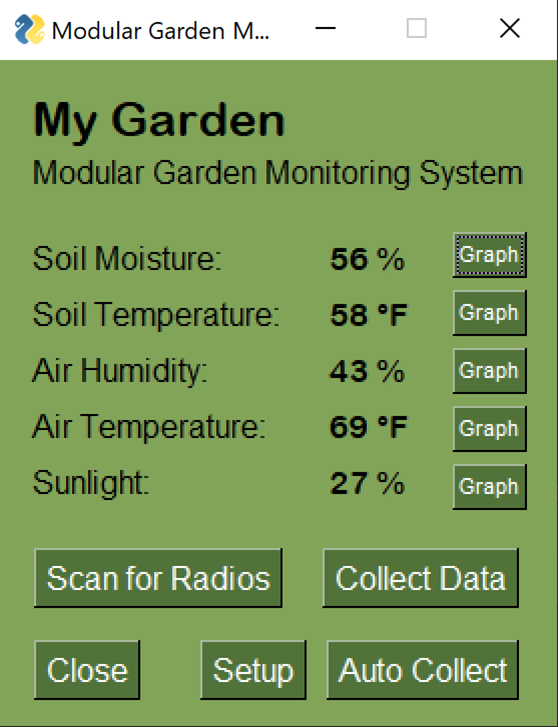
\includegraphics[height=3.5in]{PNGs/GUI.png}
    \caption{Initial GUI design}
    \label{fig:GUI}
\end{figure}

\begin{figure}[H] %H means keep figure here
    \centering
    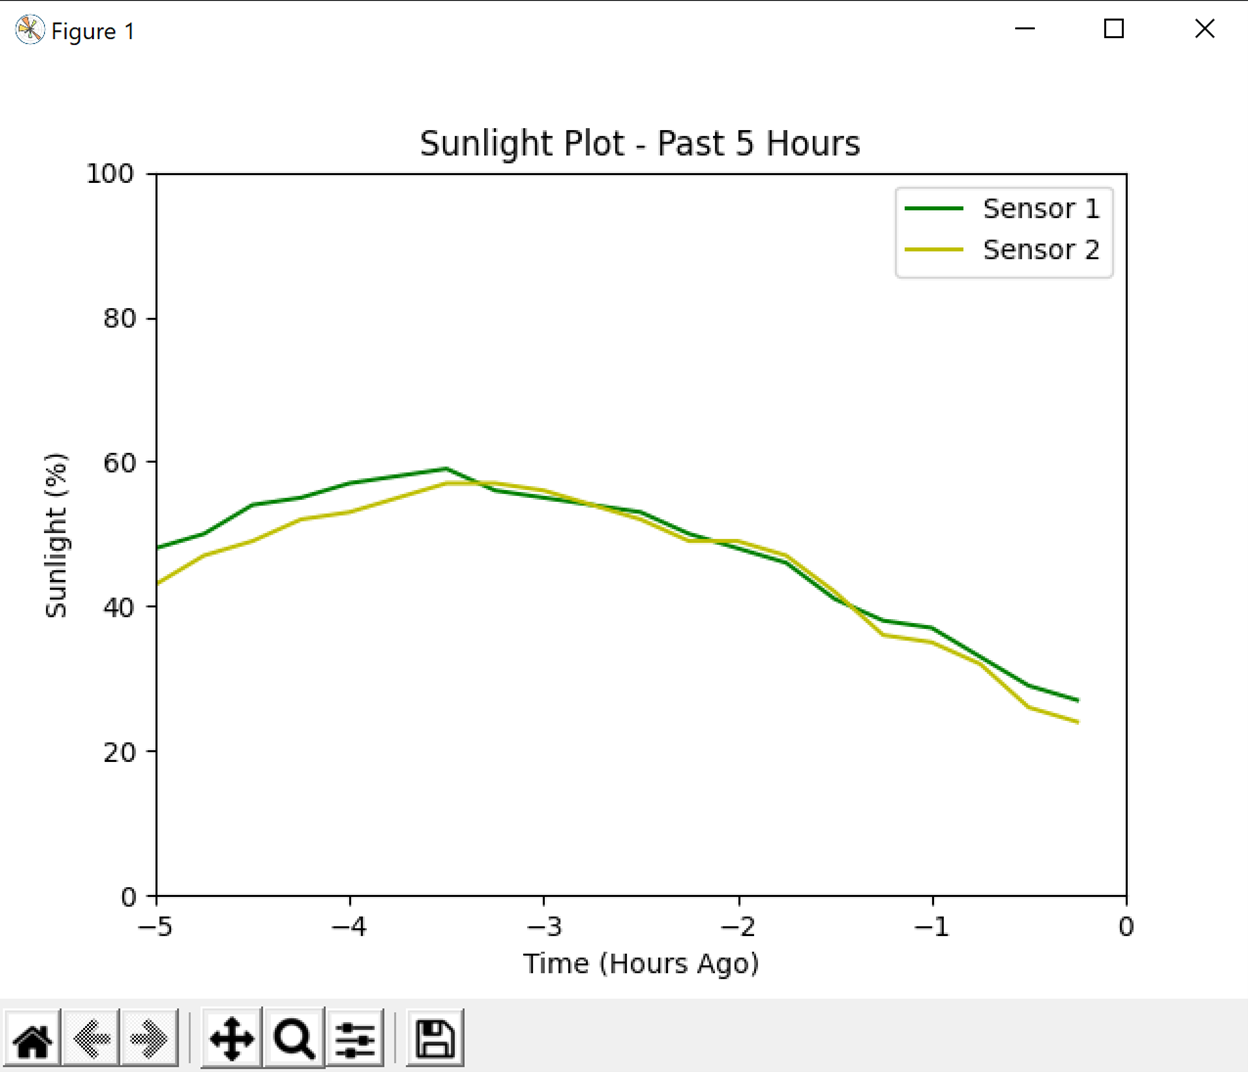
\includegraphics[height=3.5in]{PNGs/GUIGRaph.png}
    \caption{GUI Data Display in Graph Form}
    \label{fig:Graph}
\end{figure}

\newpage
Once a working prototype was developed, steps were taken to design a preliminary production design for the MGMS hardware. Due to time and software tool constraints, only production hardware for the MGMS sensor module was designed. By following the developed prototype and decomposing the open-source arduino uno and XBee platforms, a master hardware schematic was created in Altium Designer and is shown in Figure \ref{fig:Schematic}. This schematic is then used to design a printed circuit board design to support the system hardware components. This PCB is shown in Figure \ref{fig:PCB}.\\

\begin{figure}[H] %H means keep figure here
    \centering
    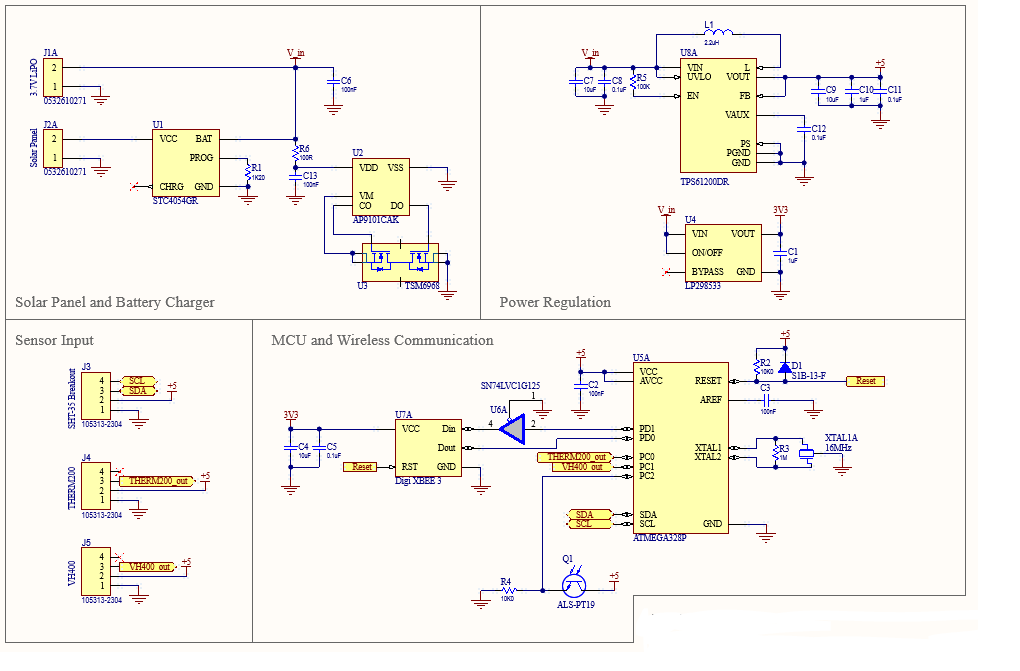
\includegraphics[height=4in]{PNGs/Schematic.PNG}
    \caption{Hardware Sensor Module Schematic.}
    \label{fig:Schematic}
\end{figure}
\begin{figure}[H] %H means keep figure here
    \centering
    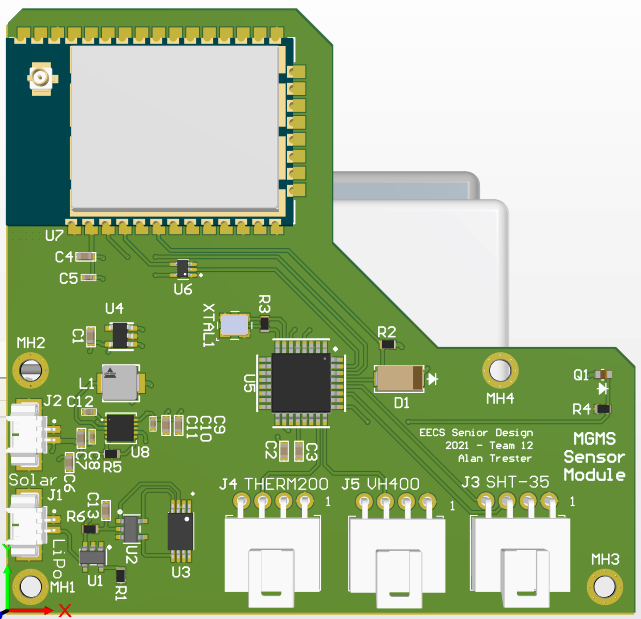
\includegraphics[height=4in]{PNGs/PCB.PNG}
    \caption{Printed Circuit Board Model for the Hardware Sensor Module.}
    \label{fig:PCB}
\end{figure}

The printed circuit board was designed in such a way that it could snugly fit into a standard transparent weatherproof container, interfaced with a standard sized solar panel and lithium-ion battery pack. The system's sunlight sensor and radio antenna are cleverly positioned as to not be obstructed by other system components. A final 3d mockup of the entire hardware stack is shown in Figure \ref{fig:Stackup}\\

\begin{figure}[H] %H means keep figure here
    \centering
    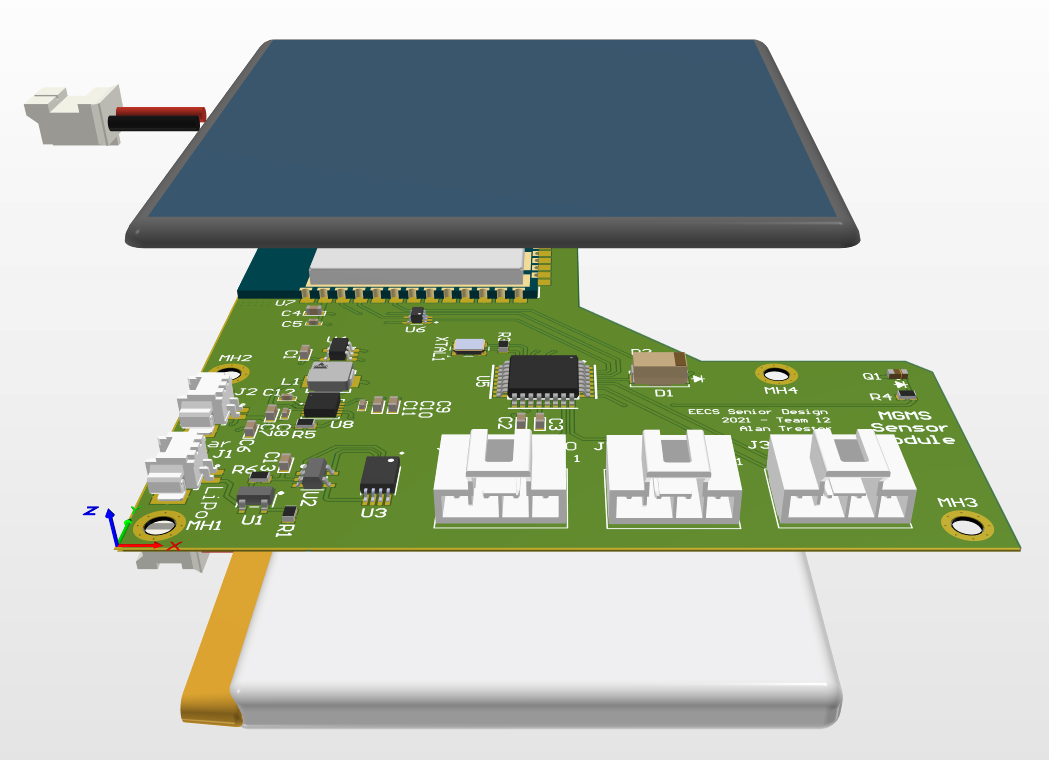
\includegraphics[height=3.25in]{PNGs/FinalAssy.PNG}
    \caption{Stack Mockup for the Hardware Sensor Module.}
    \label{fig:Stackup}
\end{figure}

\newpage
\section{Testing and System Performance}

The process of testing and confirming performance of the system's hardware components occurred subsequently with the prototype development. As each individual sensor was interfaced, calibration and speed testing occurred so that embedded software could be developed accordingly. Throughout this process, sensor accuracy and the system response time was confirmed to perform within and exceeding team expectations. Figures \ref{fig:SoilMoist}, \ref{fig:SoilTest}, and \ref{fig:AirTemp} show data used for confirming system performance of the MGMS sensor hardware module.\\

\begin{figure}[H] %H means keep figure here
    \centering
    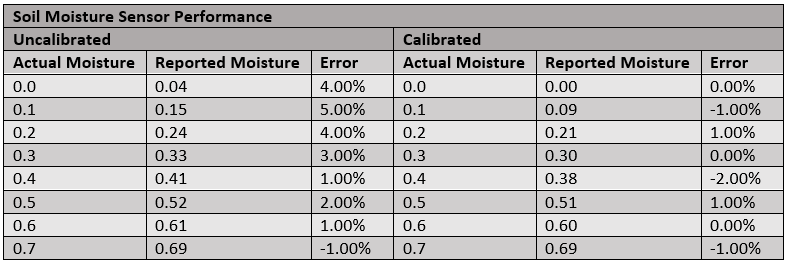
\includegraphics{PNGs/SoilMoistData.PNG}
    \caption{Soil moisture data reported by the VH400 sensor during calibration testing.}
    \label{fig:SoilMoist}
\end{figure}

\begin{figure}[H] %H means keep figure here
    \centering
    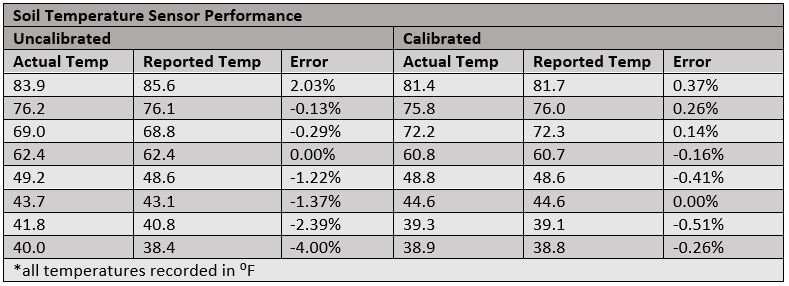
\includegraphics{PNGs/SoilTempData.PNG}
    \caption{Soil temperature data reported by the THERM200 sensor during calibration testing.}
    \label{fig:SoilTemp}
\end{figure}

\begin{figure}[H] %H means keep figure here
    \centering
    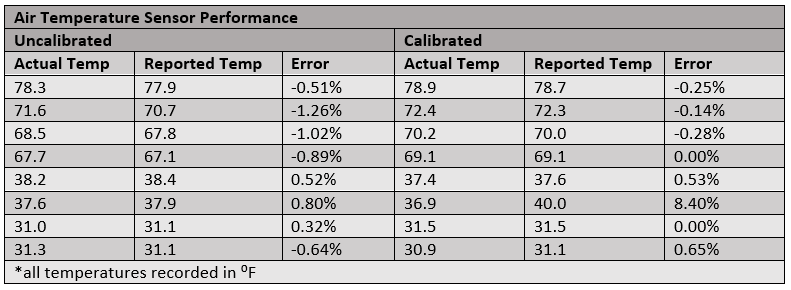
\includegraphics{PNGs/AirTempData.PNG}
    \caption{Air temperature data reported by the SHT35 sensor during calibration testing.}
    \label{fig:AirTemp}
\end{figure}

When designing the software and GUI, like the hardware components, a test driven development method was approached. Tests for the GUI and software were developed and ensured all front-end functionality would fit software capabilities. Figure \ref{fig:GUITest} illustrates key features whose performance was evaluated during the front-end development process.\\

\begin{figure}[H] %H means keep figure here
    \centering
    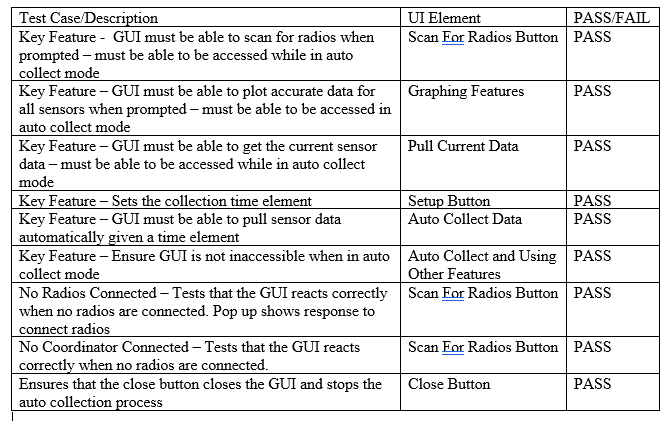
\includegraphics{PNGs/GUITestCase.PNG}
    \caption{GUI Test Case Chart shows what key features were desired from the software and how those features were tested and expected to perform.}
    \label{fig:GUITest}
\end{figure}

\newpage
\section{Budget}
The expected project budget changed over time as decisions in design and development processes were made. A finalized budget is shown below as a Bill of Materials (BoM) for the system prototype in Figure \ref{fig:bom}. This bill of materials shows costs for specific prototyping components and not necessarily the tools or work hours used to create the system. An estimated final system cost is provided based on information available from the computer aided design software and printed circuit board retailers.
\begin{figure}[H]
    \centering
    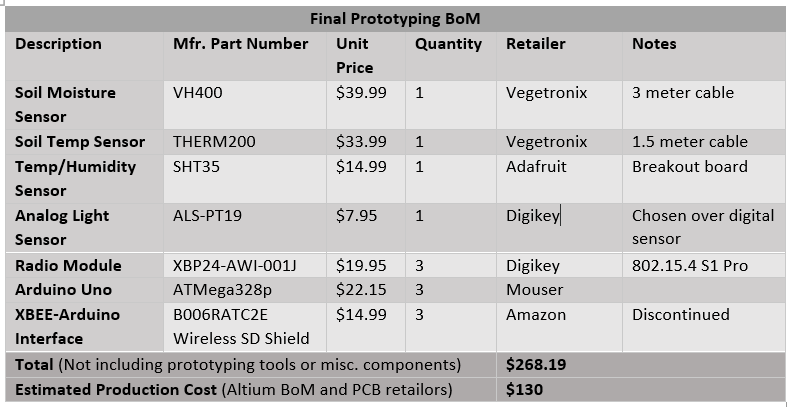
\includegraphics[width=15cm]{PNGs/BoM.PNG}
    \caption{Final prototyping Bill of Materials. Includes an estimated final system production cost}
    \label{fig:bom}
\end{figure}



\ganttset{calendar week text={\currentweek}} % set gantt scaling
% change page size and margin
\clearpage
\KOMAoptions{paper=a3, paper=landscape}
\addtolength{\hoffset}{-3.0cm}
\recalctypearea
\thispagestyle{empty}
\subsection*{Implementation}
\subsubsection*{Time}
The team plans to meet weekly using the Microsoft Teams videoconferencing application. This weekly meeting will occur every Tuesday for approximately 30 minutes starting at 3:30pm, and the work itself will be documented and shared using Teams and GitHub. The scheduled timeline is illustrated in a Gantt chart shown below. Tasks regarding the Implementation, Testing and Delivery phases are not reduced in detail as they depend on the result of the Design phase. \\

\begin{ganttchart}[
		% Gantt chart configuration
		bar/.style={fill=gray!50, draw},
		bar incomplete/.style={/pgfgantt/bar, fill=white}, % greyscale
		x unit=1.2mm, % suitable width for a3
		y unit chart=0.6cm, % smaller line spacing
		time slot format=isodate, time slot unit=day, % set gantt scaling
		progress=today, today={2020-09-24}, % auto-calculate progress
	]{2020-08-24}{2021-04-29} % start of fall 2020 to end of fall 2021
	\gantttitlecalendar{year, month=shortname} \\ % title config
	%%%%%%%%%%%%%%%%%%%%%%%%%%%%%%%%%%%%%%%%%%%%%%%%%%%%%%%%%%%%%%%%%%%%
	%                   Edit here to update tasks                      %
	%%%%%%%%%%%%%%%%%%%%%%%%%%%%%%%%%%%%%%%%%%%%%%%%%%%%%%%%%%%%%%%%%%%%
	% Format:
	% \gantbar{task-name}{startyear-month-day}{endyear-month-day} \\

	% No need to input progress, it calculates progress when built ヽ( •_)ᕗ
	% Don't forget to new line at the end!
	\ganttgroup{Definition}{2020-08-24}{2020-09-27} \\
	\ganttbar{Rough system diagram}{2020-08-24}{2020-09-18} \\
	\ganttbar{Final preliminary system design}{2020-09-18}{2020-09-27} \\
	\ganttbar{Bill of Material}{2020-09-18}{2020-09-27} \\

	\ganttgroup{Design}{2020-09-27}{2020-11-15} \\
	\ganttbar{Order parts}{2020-09-27}{2020-11-15} \\
	\ganttbar{Front end development}{2020-09-27}{2020-11-08} \\
	\ganttbar{Firmware development}{2020-09-27}{2020-11-08} \\
	\ganttbar{Control system development}{2020-09-27}{2020-11-15} \\
	\ganttbar{System Prototype}{2020-11-01}{2020-11-15} \\
	\ganttbar{Additional hardware}{2020-10-15}{2020-11-01} \\

	\ganttgroup{Implementation}{2020-11-01}{2020-12-31} \\
	%\ganttbar{Finalize UI}{}{}
	%\ganttbar{Finalize and order PCB}{}{}
	%\ganttbar{System assembly}{}{}

	\ganttgroup{Testing}{2021-01-01}{2021-02-28} \\


	\ganttgroup{Delivery}{2021-03-01}{2021-04-29} \\









\end{ganttchart}
%%%%%%%%%%%%%%%%%%%%%%%%%%%%%%%%%%%%%%%%%%%%%%%%%%%%%%%%%%%%%%%%%%%%
%                       Gantt Chart Ends                           %
%%%%%%%%%%%%%%%%%%%%%%%%%%%%%%%%%%%%%%%%%%%%%%%%%%%%%%%%%%%%%%%%%%%%
\vfill
\begin{center}
	\hspace{5.0cm}
	\thepage
\end{center}


% restore page size and margin
\clearpage
\KOMAoptions{paper=a4, paper=portrait}
\recalctypearea
\addtolength{\hoffset}{+3.0cm}

% restore page size and margin
\clearpage
\KOMAoptions{paper=a4, paper=portrait}
\recalctypearea
\addtolength{\hoffset}{+4.0cm}

Throughout the course of the project, it was estimated that each individual person on the team would work approximately 7-10 hours per week. Some weeks will be lighter on work (waiting for parts to be shipped), while others will be more labor intensive (assembly and programming), but overall the estimate of 7-10 hours per week is a fair number. Below is a rough chart documenting the overall time spent working on the project, which supplements the information shown in the Gantt Chart in the previous section.\\

\begin{figure}[H]
    \centering
    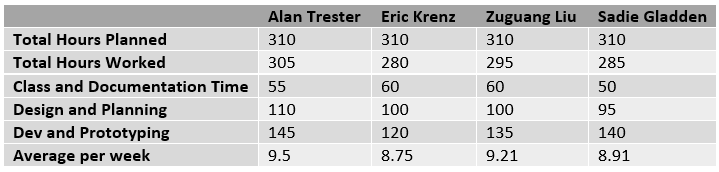
\includegraphics[width=15cm]{PNGs/TimeChart.PNG}
    \caption{Time Chart showing the allocation of past time spent and future time expected  on the project.}
    \label{fig:time_chart}
\end{figure}

Just like the Gantt Chart, this table was continually updated as the project progressed.

\section{Problems Encountered and Solutions}

The COVID-19 pandemic in 2020 and 2021 changed many of the ways that world operates. Just as the global pandemic was unprecedented, many of the changes that students at the University of Cincinnati faced have also been unprecedented. Many new challenges, on top of the ones that are typically faced arose during this academic year which changed that way that this senior design project was approached.\\

The biggest challenge for the team as a result of the global pandemic was the requirement for virtual collaboration as opposed to in-person meetings. Working and collaborating virtually for class sessions as well as group work often hindered progress and communication since instant feedback was not always available as it may have been otherwise. Typically, staying updated on class assignments, keeping track of team progress, and having multiple people collaborate on one project component were uniquely difficult processes. The team adjusted to the new reality in several ways, the most important of which was perhaps by taking advantage of new collaboration and planning tools to complete documentation and project tasks. Tools such as Microsoft Teams, Overleaf, and GIT were leveraged much more heavily than they would have otherwise. Additionally, as a result of the virtual environment, the team did not have access to EECS collaboration spaces and electronic labs, instead working from home offices without the tools, equipment, and real-time team input that otherwise would have been available. Instead, our home offices had to be turned into personal lab spaces by acquiring equipment such as oscilloscopes, multimeters, and 3D printers to use for project development. Lastly, project funding, which is typically provided by EECS, was made unavailable, which further hindered development efforts.\\

One typical challenge that arose for our team was development with outdated and obsolete technology. Due to personal budget constraints, several system components were chosen due to their existing availability to use in project development. In particular, the XBEE S1 Pro radios which were used to build the MGMS's wireless communication system used an outdated IEEE 802.15.4 firmware that has been replaced in the 2nd, 3rd, and 4th generation XBEE radios with Zigbee and Digimesh features. Working with an outdated technology limited certain system functionalities that would have proved useful for system development. Furthermore, because we are designing the system in such a way that it can be wholly produced, we had to cleverly develop the system prototype in such a way that functionality would be forward-compatible with the newer technology that would likely be used.

\section{Future Recommendations}
In the future, there are many possibilities and opportunities to improve upon this prototype. Of course, this is a baseline proof-of-concept system which can be ever-improved with more developed features on top of the system platforms that have been created. Although the platform was designed in a way that could easily accommodate these features, time constraints prevented more sophisticated user interaction and internet connectivity features from being fully realized. Time and equipment constraints also prevented the team from wholly testing the completed prototype. Although the system functioned as expected, it was impossible to measure the hardware and software limits to be documented for further development. Had testing been planned well in advance, this information may have been more attainable and used to create a better final product. The final system can be expanded to be significantly more impressive through designing simple components such as solenoid valve units for watering. It is arguable that it would be possible to create a more well-rounded demonstrable product if less time was spent on the hardware development of the main sensor module.

%%%%%%%%%%%%%%%%%%%%%%%%%%%%%%%%%%%%%%%%%%%%%%%%%%%%%%%%%%%%%%%%%%%%%%
%Conclusion
%%%%%%%%%%%%%%%%%%%%%%%%%%%%%%%%%%%%%%%%%%%%%%%%%%%%%%%%%%%%%%%%%%%%%%
\chapter{Conclusion}
In completing our senior design project we were able to successfully design, prototype, and test the proof-of-concept garden monitoring system to the expectations laid out in the initial design plans. The presented MGMS prototype demonstrates the core system functionality: a thoroughly developed and easy to interface modular wireless communication system, accurate environmental readings, efficient communication, and a robust user interface platform. The time and effort spent developing our core system components means that the development of new features and hardware can be streamlined. With time, a full, marketable, consumer-grade system can be built that effectively promotes green spaces and addresses the water conservation concerns that are brought up at the beginning of this report, filling a very important market space. Considering the previously discussed challenges, solutions, and proposed improvements, our team has a very optimistic outlook on the future of the MGMS system if it were to be further developed.\\\\

%MAKE THIS DO THINGS
\bibliography{bibliography}
\bibliographystyle{ieeetr}

\newpage
\chapter{Appendices}
% subsection for "Python Code for GUI" included in pycode.tex
\section{Python Implementation of GUI}
\lstinputlisting[language=Python]{../../code/python-gui/mgms.py}

\newpage
\section{Submodule Main Control Program}
\lstinputlisting[language=C]{../../code/cpp-sensor-module/MGMS-Sensor-Module/main.cpp}

\newpage
\section{Submodule Libraries}
\lstinputlisting[language=C]{../../code/cpp-sensor-module/MGMS-Sensor-Module/SHT35.h}
\lstinputlisting[language=C]{../../code/cpp-sensor-module/MGMS-Sensor-Module/SHT35.cpp}
\newpage
\lstinputlisting[language=C]{../../code/cpp-sensor-module/MGMS-Sensor-Module/twi_lib.h}
\lstinputlisting[language=C]{../../code/cpp-sensor-module/MGMS-Sensor-Module/twi_lib.cpp}
\newpage
\lstinputlisting[language=C]{../../code/cpp-sensor-module/MGMS-Sensor-Module/AnalogSensors.h}
\lstinputlisting[language=C]{../../code/cpp-sensor-module/MGMS-Sensor-Module/AnalogSensors.cpp}

\end{document}